\newpage

The following article is reproduced from \textcite{Zeitlin-2018} with permission from Geophysical Research Letters, \copyright American Geophysical Union:\\

\pubcite{Guo-2018}
\hfill Own contribution: 10\%

\newpage
\newcounter{includepdfpageGuoEighteen}

\addtocounter{section}{1}
\setcounter{subsection}{1} 
\phantomsection
\addcontentsline{toc}{section}{\arabic{chapter}.\arabic{section} Modeling the Evolution and Propagation of 10 September 2017 CMEs and SEPs Arriving at Mars Constrained by Remote Sensing and In Situ Measurement (Publication Space Weather 2018)}
%
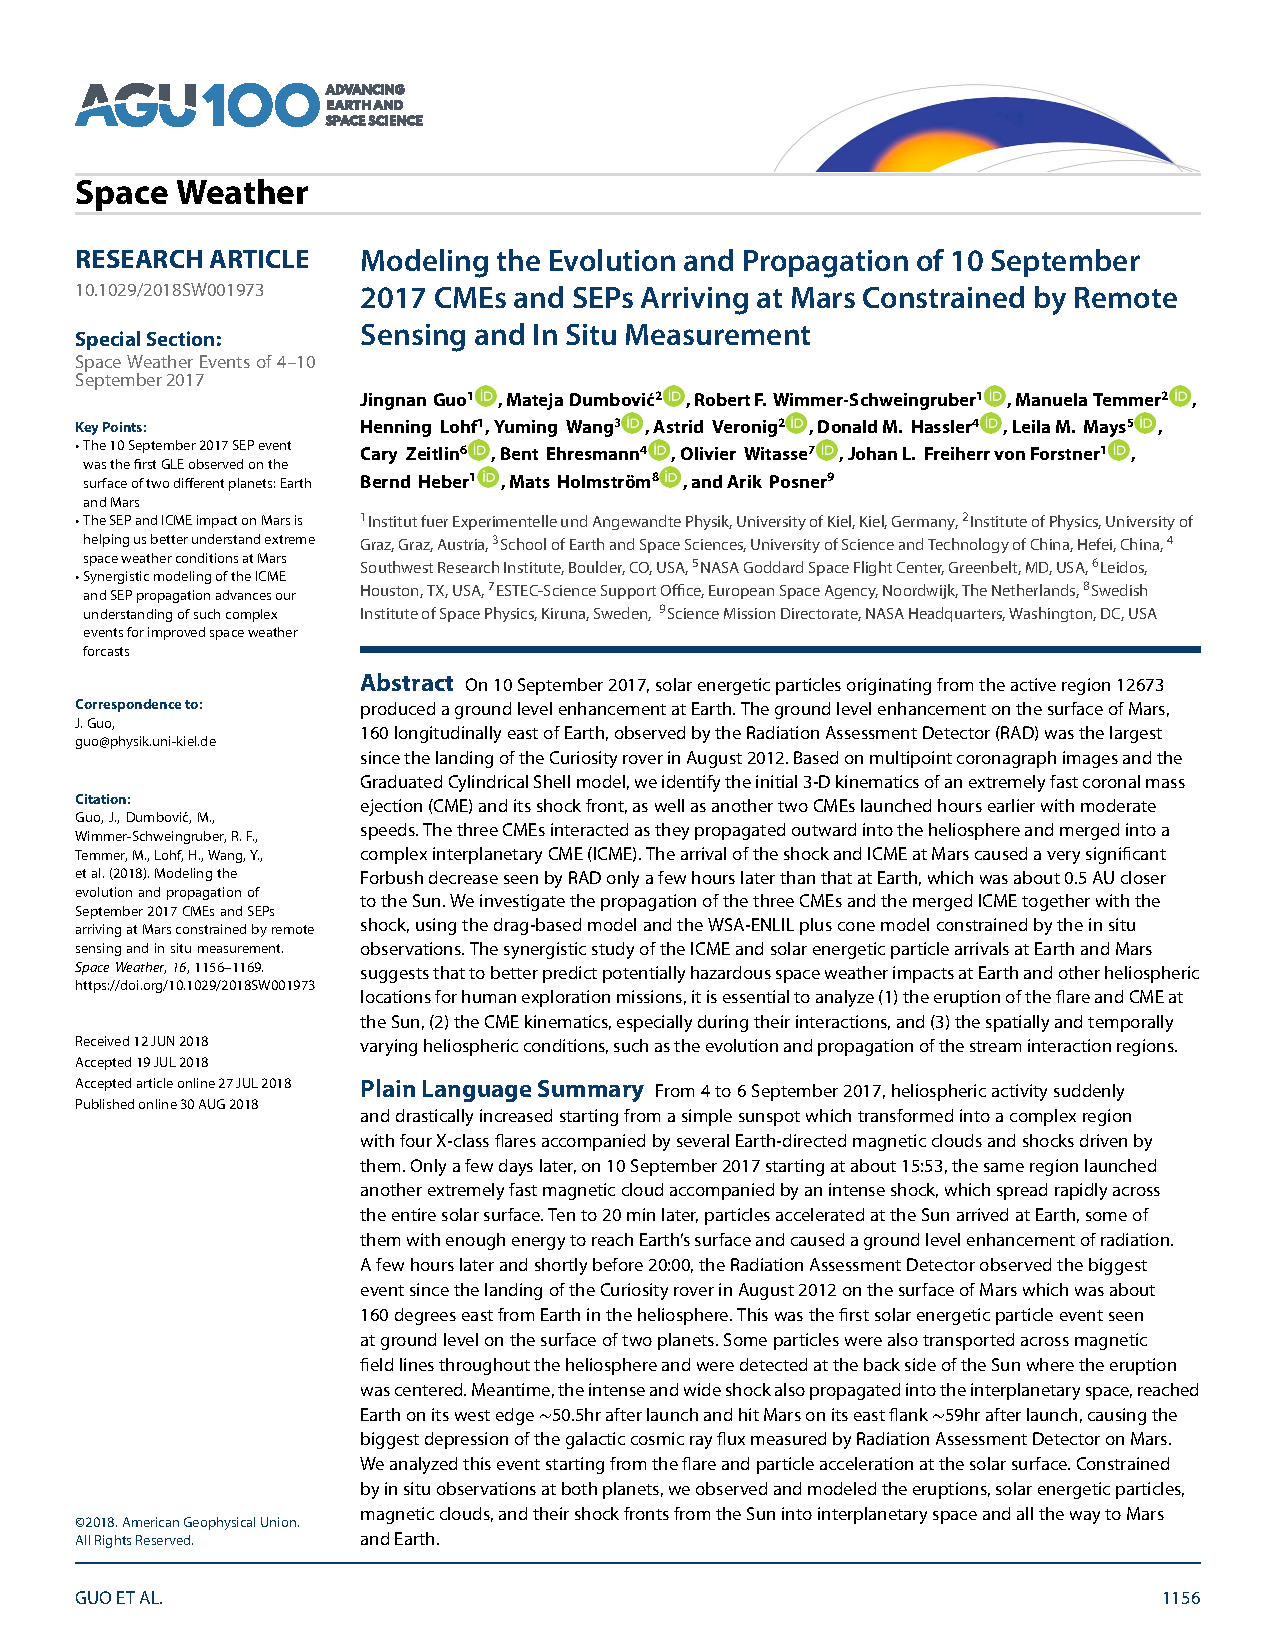
\includepdf[pages={1}, link, linkname=paper_guo2018, scale=.95, pagecommand={\refstepcounter{includepdfpageGuoEighteen}\label{paper_guo2018.\theincludepdfpageGuoEighteen}}]{publications/Guo_et_al-2018-Space_Weather}
%
\phantomsection
\addcontentsline{toc}{subsection}{\arabic{chapter}.\arabic{section}.\arabic{subsection} The Flare, CMEs, and GLE 72: Close to the Sun}
\label{sec:paper_guo2018}
%
\includepdf[pages={2-4}, link, linkname=paper_guo2018, scale=.95, pagecommand={\refstepcounter{includepdfpageGuoEighteen}\label{paper_guo2018.\theincludepdfpageGuoEighteen}}]{publications/Guo_et_al-2018-Space_Weather}
%
\addtocounter{subsection}{1} 
\phantomsection
\addcontentsline{toc}{subsection}{\arabic{chapter}.\arabic{section}.\arabic{subsection} The Interplanetary Trajectory and Interaction of Three CMEs Modeled by the DBM}
\includepdf[pages={5-6}, link, linkname=paper_guo2018, scale=.95, pagecommand={\refstepcounter{includepdfpageGuoEighteen}\label{paper_guo2018.\theincludepdfpageGuoEighteen}}]{publications/Guo_et_al-2018-Space_Weather}
%
\addtocounter{subsection}{1} 
\phantomsection
\addcontentsline{toc}{subsection}{\arabic{chapter}.\arabic{section}.\arabic{subsection} Shock Kinematics and Propagation Toward Earth and Mars: Data-Constrained DBM}
\includepdf[pages={7}, link, linkname=paper_guo2018, scale=.95, pagecommand={\refstepcounter{includepdfpageGuoEighteen}\label{paper_guo2018.\theincludepdfpageGuoEighteen}}]{publications/Guo_et_al-2018-Space_Weather}
%
\addtocounter{subsection}{1} 
\phantomsection
\addcontentsline{toc}{subsection}{\arabic{chapter}.\arabic{section}.\arabic{subsection} The Shock and ICME Arrival at Mars and Earth: Modeled Results and In Situ Observations}
\includepdf[pages={8}, link, linkname=paper_guo2018, scale=.95, pagecommand={\refstepcounter{includepdfpageGuoEighteen}\label{paper_guo2018.\theincludepdfpageGuoEighteen}}]{publications/Guo_et_al-2018-Space_Weather}
%
\addtocounter{subsection}{1} 
\phantomsection
\addcontentsline{toc}{subsection}{\arabic{chapter}.\arabic{section}.\arabic{subsection} SEPs Arriving at Earth, Mars, and STA and the Indication of the Shockand Stream Interaction Region Propagation}
\includepdf[pages={9-10}, link, linkname=paper_guo2018, scale=.95, pagecommand={\refstepcounter{includepdfpageGuoEighteen}\label{paper_guo2018.\theincludepdfpageGuoEighteen}}]{publications/Guo_et_al-2018-Space_Weather}
%
\addtocounter{subsection}{1} 
\phantomsection
\addcontentsline{toc}{subsection}{\arabic{chapter}.\arabic{section}.\arabic{subsection} Summary and Conclusion}
\includepdf[pages={11}, link, linkname=paper_guo2018, scale=.95, pagecommand={\refstepcounter{includepdfpageGuoEighteen}\label{paper_guo2018.\theincludepdfpageGuoEighteen}}]{publications/Guo_et_al-2018-Space_Weather}
%
\addtocounter{subsection}{1} 
\phantomsection
\addcontentsline{toc}{subsection}{\arabic{chapter}.\arabic{section}.\arabic{subsection} Appendix A: References of the Measurements and Databases Employed in This Study}
\includepdf[pages={12}, link, linkname=paper_guo2018, scale=.95, pagecommand={\refstepcounter{includepdfpageGuoEighteen}\label{paper_guo2018.\theincludepdfpageGuoEighteen}}]{publications/Guo_et_al-2018-Space_Weather}
%
\addtocounter{subsection}{1} 
\phantomsection
\addcontentsline{toc}{subsection}{\arabic{chapter}.\arabic{section}.\arabic{subsection} References}
\includepdf[pages={13-14}, link, linkname=paper_guo2018, scale=.95, pagecommand={\refstepcounter{includepdfpageGuoEighteen}\label{paper_guo2018.\theincludepdfpageGuoEighteen}}]{publications/Guo_et_al-2018-Space_Weather}